\documentclass[twoside]{book}

% Packages required by doxygen
\usepackage{fixltx2e}
\usepackage{calc}
\usepackage{doxygen}
\usepackage[export]{adjustbox} % also loads graphicx
\usepackage{graphicx}
\usepackage[utf8]{inputenc}
\usepackage{makeidx}
\usepackage{multicol}
\usepackage{multirow}
\PassOptionsToPackage{warn}{textcomp}
\usepackage{textcomp}
\usepackage[nointegrals]{wasysym}
\usepackage[table]{xcolor}

% Font selection
\usepackage[T1]{fontenc}
\usepackage[scaled=.90]{helvet}
\usepackage{courier}
\usepackage{amssymb}
\usepackage{sectsty}
\renewcommand{\familydefault}{\sfdefault}
\allsectionsfont{%
  \fontseries{bc}\selectfont%
  \color{darkgray}%
}
\renewcommand{\DoxyLabelFont}{%
  \fontseries{bc}\selectfont%
  \color{darkgray}%
}
\newcommand{\+}{\discretionary{\mbox{\scriptsize$\hookleftarrow$}}{}{}}

% Page & text layout
\usepackage{geometry}
\geometry{%
  a4paper,%
  top=2.5cm,%
  bottom=2.5cm,%
  left=2.5cm,%
  right=2.5cm%
}
\tolerance=750
\hfuzz=15pt
\hbadness=750
\setlength{\emergencystretch}{15pt}
\setlength{\parindent}{0cm}
\setlength{\parskip}{3ex plus 2ex minus 2ex}
\makeatletter
\renewcommand{\paragraph}{%
  \@startsection{paragraph}{4}{0ex}{-1.0ex}{1.0ex}{%
    \normalfont\normalsize\bfseries\SS@parafont%
  }%
}
\renewcommand{\subparagraph}{%
  \@startsection{subparagraph}{5}{0ex}{-1.0ex}{1.0ex}{%
    \normalfont\normalsize\bfseries\SS@subparafont%
  }%
}
\makeatother

% Headers & footers
\usepackage{fancyhdr}
\pagestyle{fancyplain}
\fancyhead[LE]{\fancyplain{}{\bfseries\thepage}}
\fancyhead[CE]{\fancyplain{}{}}
\fancyhead[RE]{\fancyplain{}{\bfseries\leftmark}}
\fancyhead[LO]{\fancyplain{}{\bfseries\rightmark}}
\fancyhead[CO]{\fancyplain{}{}}
\fancyhead[RO]{\fancyplain{}{\bfseries\thepage}}
\fancyfoot[LE]{\fancyplain{}{}}
\fancyfoot[CE]{\fancyplain{}{}}
\fancyfoot[RE]{\fancyplain{}{\bfseries\scriptsize Generated by Doxygen }}
\fancyfoot[LO]{\fancyplain{}{\bfseries\scriptsize Generated by Doxygen }}
\fancyfoot[CO]{\fancyplain{}{}}
\fancyfoot[RO]{\fancyplain{}{}}
\renewcommand{\footrulewidth}{0.4pt}
\renewcommand{\chaptermark}[1]{%
  \markboth{#1}{}%
}
\renewcommand{\sectionmark}[1]{%
  \markright{\thesection\ #1}%
}

% Indices & bibliography
\usepackage{natbib}
\usepackage[titles]{tocloft}
\setcounter{tocdepth}{3}
\setcounter{secnumdepth}{5}
\makeindex

% Hyperlinks (required, but should be loaded last)
\usepackage{ifpdf}
\ifpdf
  \usepackage[pdftex,pagebackref=true]{hyperref}
\else
  \usepackage[ps2pdf,pagebackref=true]{hyperref}
\fi
\hypersetup{%
  colorlinks=true,%
  linkcolor=blue,%
  citecolor=blue,%
  unicode%
}

% Custom commands
\newcommand{\clearemptydoublepage}{%
  \newpage{\pagestyle{empty}\cleardoublepage}%
}

\usepackage{caption}
\captionsetup{labelsep=space,justification=centering,font={bf},singlelinecheck=off,skip=4pt,position=top}

%===== C O N T E N T S =====

\begin{document}

% Titlepage & ToC
\hypersetup{pageanchor=false,
             bookmarksnumbered=true,
             pdfencoding=unicode
            }
\pagenumbering{roman}
\begin{titlepage}
\vspace*{7cm}
\begin{center}%
{\Large B\+FS module }\\
\vspace*{1cm}
{\large Generated by Doxygen 1.8.11}\\
\end{center}
\end{titlepage}
\clearemptydoublepage
\tableofcontents
\clearemptydoublepage
\pagenumbering{arabic}
\hypersetup{pageanchor=true}

%--- Begin generated contents ---
\chapter{Breadth First Search (B\+FS)}
\label{md__home_shivang_Desktop_808x_rough_files_week_6_808x_midterm_project_readme}
\hypertarget{md__home_shivang_Desktop_808x_rough_files_week_6_808x_midterm_project_readme}{}
\href{https://travis-ci.org/shivaang12/808x_midterm_project}{\tt } \href{https://coveralls.io/github/shivaang12/808x_midterm_project?branch=master}{\tt } \href{https://opensource.org/licenses/MIT}{\tt }

\subsection*{Overview}

A basic planner module for any traversable vehicle by Acme Robotics. Acme\textquotesingle{}s high level planner sometimes need local planner for estimating feasible paths for the robot. This planner, given the information of the environment, starting point and goal point, will provide feasible path from start point to goal point. It will executes Breath First Search algorithm to find feasible path between start point and goal point. More details can be found below.

\subsection*{Dependencies}

To build and run this module successfully, following dependencies should be met\+:
\begin{DoxyItemize}
\item C\+Make version at least 3.\+2.\+1
\item S\+DL 2.\+0.\+8 or higher\+: To download and build the library, please follow the instructions 
\begin{DoxyCode}
1 curl -L https://www.libsdl.org/release/SDL2-2.0.8.tar.gz | tar xz cd SDL2-2.0.8
2 ./configure
3 make
4 sudo make install
\end{DoxyCode}

\item For unit testing, this project depends on {\itshape gtest} framework by Google.
\end{DoxyItemize}

\#\# Instructions to build the module 
\begin{DoxyCode}
1 git clone --recursive https://github.com/shivaang12/808x\_midterm\_project
2 cd <path to repository>
3 mkdir build
4 cd build
5 cmake ..
6 make
7 Run tests: ./test/cpp-test
8 Run program: ./app/shell-app
\end{DoxyCode}


\subsection*{Algorithm}

Breath First Search algorithm is essentially a search algorithm. It is mostly used for traversing in robotics. Algorithm intitally start from a start point by adding to a priority queue. Then it explores each node from a priority queue to its child and adds to to a priority queue till it encounters goal point. In between, algorithm links each node to its respective childs. If it encounters goal point during exploration, then this links will be used to link back to start point. This will be the feasible path from start point to goal point generated using B\+FS algorithm.

\subsection*{Output}

Given the start point -\/$>$ (0, 599) and goal point -\/$>$ (799, 0), below is the output figure. \tabulinesep=1mm
\begin{longtabu} spread 0pt [c]{*1{|X[-1]}|}
\hline
\rowcolor{\tableheadbgcolor}{\bf Output Image  }\\\cline{1-1}
\endfirsthead
\hline
\endfoot
\hline
\rowcolor{\tableheadbgcolor}{\bf Output Image  }\\\cline{1-1}
\endhead
 \\\cline{1-1}
\end{longtabu}
\subsection*{Singular Iterative Process (S\+IP)}

S\+IP process charts for this project can be found \href{https://docs.google.com/spreadsheets/d/1IbgtYZAE8amdw-byhspCRRnXf8tBoE707xSWsrF4pjw/edit?usp=sharing}{\tt here}. 
\chapter{Class Index}
\section{Class List}
Here are the classes, structs, unions and interfaces with brief descriptions\+:\begin{DoxyCompactList}
\item\contentsline{section}{\hyperlink{class_bfs}{Bfs} \\*\hyperlink{class_bfs}{Bfs} class which is used to find stortest path possible by using B\+FS algorithm }{\pageref{class_bfs}}{}
\item\contentsline{section}{\hyperlink{class_obstacle__generator}{Obstacle\+\_\+generator} \\*This class will mimic the Acme\textquotesingle{}s high level planner\textquotesingle{}s . This class will provide the hight and width of the area, obstacle space and start -\/ goal points. And evoke the planner }{\pageref{class_obstacle__generator}}{}
\item\contentsline{section}{\hyperlink{class_sdl__wrapper}{Sdl\+\_\+wrapper} \\*S\+DL library wrapper class for visulization of the B\+FS algorithm through the \hyperlink{class_bfs}{Bfs} class. This class will accept all the information regarding the environment and path for plotting them in nice visuals }{\pageref{class_sdl__wrapper}}{}
\end{DoxyCompactList}

\chapter{File Index}
\section{File List}
Here is a list of all documented files with brief descriptions\+:\begin{DoxyCompactList}
\item\contentsline{section}{/home/shivang/\+Desktop/808x/rough\+\_\+files/week\+\_\+6/808x\+\_\+midterm\+\_\+project/app/\hyperlink{bfs_8cpp}{bfs.\+cpp} \\*D\+E\+S\+C\+R\+I\+P\+T\+I\+ON This file implements \hyperlink{class_bfs}{Bfs} class }{\pageref{bfs_8cpp}}{}
\item\contentsline{section}{/home/shivang/\+Desktop/808x/rough\+\_\+files/week\+\_\+6/808x\+\_\+midterm\+\_\+project/app/\hyperlink{main_8cpp}{main.\+cpp} \\*D\+E\+S\+C\+R\+I\+P\+T\+I\+ON This files is the main file which creates object of \hyperlink{class_obstacle__generator}{Obstacle\+\_\+generator} class }{\pageref{main_8cpp}}{}
\item\contentsline{section}{/home/shivang/\+Desktop/808x/rough\+\_\+files/week\+\_\+6/808x\+\_\+midterm\+\_\+project/app/\hyperlink{obstacle__generator_8cpp}{obstacle\+\_\+generator.\+cpp} \\*D\+E\+S\+C\+R\+I\+P\+T\+I\+ON This files implements the class \hyperlink{class_obstacle__generator}{Obstacle\+\_\+generator} }{\pageref{obstacle__generator_8cpp}}{}
\item\contentsline{section}{/home/shivang/\+Desktop/808x/rough\+\_\+files/week\+\_\+6/808x\+\_\+midterm\+\_\+project/app/\hyperlink{sdl__wrapper_8cpp}{sdl\+\_\+wrapper.\+cpp} \\*D\+E\+S\+C\+R\+I\+P\+T\+I\+ON This files implements the class \hyperlink{class_sdl__wrapper}{Sdl\+\_\+wrapper} }{\pageref{sdl__wrapper_8cpp}}{}
\item\contentsline{section}{/home/shivang/\+Desktop/808x/rough\+\_\+files/week\+\_\+6/808x\+\_\+midterm\+\_\+project/include/\hyperlink{bfs_8hpp}{bfs.\+hpp} \\*D\+E\+S\+C\+R\+I\+P\+T\+I\+ON Header file for the class \hyperlink{class_bfs}{Bfs}. \hyperlink{class_bfs}{Bfs} class implements a planning algorithm B\+FS. Breadth First Search algorithm is used for traversing as well as searching. It starts at root and explores all the neighbor nodes at current depth before moving to next depth untill it finds the required thing, or traverse to the goal point respectively }{\pageref{bfs_8hpp}}{}
\item\contentsline{section}{/home/shivang/\+Desktop/808x/rough\+\_\+files/week\+\_\+6/808x\+\_\+midterm\+\_\+project/include/\hyperlink{obstacle__generator_8hpp}{obstacle\+\_\+generator.\+hpp} \\*D\+E\+S\+C\+R\+I\+P\+T\+I\+ON This class will artificially generate obstacle, throught methods, for B\+FS algorithm. This class will act as Acme\textquotesingle{}s high level planner\textquotesingle{}s input to \hyperlink{class_bfs}{Bfs} module }{\pageref{obstacle__generator_8hpp}}{}
\item\contentsline{section}{/home/shivang/\+Desktop/808x/rough\+\_\+files/week\+\_\+6/808x\+\_\+midterm\+\_\+project/include/\hyperlink{sdl__wrapper_8hpp}{sdl\+\_\+wrapper.\+hpp} \\*D\+E\+S\+C\+R\+I\+P\+T\+I\+ON Header file for the class \char`\"{}\+Sdl\+\_\+wrapper\char`\"{}. This class act as wrapper of original S\+DL library for C++. It encaptulates enough functionality from the library for visual of environment, on which B\+FS has been used, and path it has generated. Information about path and environment, obstacles and space size, will be recieved externally from \hyperlink{class_obstacle__generator}{Obstacle\+\_\+generator} class and this will generate visuals accordingly }{\pageref{sdl__wrapper_8hpp}}{}
\end{DoxyCompactList}

\chapter{Class Documentation}
\hypertarget{class_bfs}{}\section{Bfs Class Reference}
\label{class_bfs}\index{Bfs@{Bfs}}


\hyperlink{class_bfs}{Bfs} class which is used to find stortest path possible by using B\+FS algorithm.  




{\ttfamily \#include $<$bfs.\+hpp$>$}

\subsection*{Public Member Functions}
\begin{DoxyCompactItemize}
\item 
\hyperlink{class_bfs_a25bb98dd5a3e3ceab6940adad7e7d758}{Bfs} (int width, int height, std\+::pair$<$ int, int $>$ start\+\_\+point, std\+::pair$<$ int, int $>$ goal\+\_\+point)
\begin{DoxyCompactList}\small\item\em A constructor sets width\+\_\+, height\+\_\+, start\+\_\+point\+\_\+ and goal\+\_\+point\+\_\+ vars of the class. \end{DoxyCompactList}\item 
\hyperlink{class_bfs_a9ccaf8189ccb3f590c8ebca2d814c775}{Bfs} (int width, int height, std\+::pair$<$ int, int $>$ start\+\_\+point, std\+::pair$<$ int, int $>$ goal\+\_\+point, std\+::shared\+\_\+ptr$<$ std\+::vector$<$ int $>$$>$ occupancy\+\_\+matrix)
\begin{DoxyCompactList}\small\item\em A constructor sets width\+\_\+, height\+\_\+, start\+\_\+point\+\_\+, goal\+\_\+point\+\_\+ vars and occupancy\+\_\+matrix of the class. \end{DoxyCompactList}\item 
auto \hyperlink{class_bfs_a731c6ba80fdc5aa90d9c41e2829049a7}{set\+\_\+occmat} (std\+::shared\+\_\+ptr$<$ std\+::vector$<$ int $>$$>$ occupancy\+\_\+matrix) -\/$>$ int
\begin{DoxyCompactList}\small\item\em Sets the occupancy\+\_\+matrix\+\_\+ of the class. \end{DoxyCompactList}\item 
auto \hyperlink{class_bfs_a4c6fde0f40891f828481bb460dbca874}{set\+\_\+width} (int width) -\/$>$ void
\begin{DoxyCompactList}\small\item\em Sets the width\+\_\+ var of the class. \end{DoxyCompactList}\item 
auto \hyperlink{class_bfs_aabc02f36ad832553dcc0c7a59f4ba33f}{get\+\_\+width} (void) -\/$>$ int
\begin{DoxyCompactList}\small\item\em Getter method to retrive the width\+\_\+ var of the class. \end{DoxyCompactList}\item 
auto \hyperlink{class_bfs_afe4ec025381a484e7e44c00eefd344a5}{set\+\_\+height} (int height) -\/$>$ void
\begin{DoxyCompactList}\small\item\em Sets the height\+\_\+ var of the class. \end{DoxyCompactList}\item 
auto \hyperlink{class_bfs_ae982ad85510c5a58d8f7ae0dcd7ca0b7}{get\+\_\+height} (void) -\/$>$ int
\begin{DoxyCompactList}\small\item\em Getter method to retrive the height\+\_\+ var of the class. \end{DoxyCompactList}\item 
auto \hyperlink{class_bfs_aa593e45070cc4a6b2da2033db2807dba}{set\+\_\+startpoint} (std\+::pair$<$ int, int $>$ start\+\_\+point) -\/$>$ void
\begin{DoxyCompactList}\small\item\em Sets the start\+\_\+point\+\_\+ var of the class. \end{DoxyCompactList}\item 
auto \hyperlink{class_bfs_a2135a092516b1a479fcb0ab2c29d7c6b}{get\+\_\+startpoint} (void) -\/$>$ std\+::pair$<$ int, int $>$
\begin{DoxyCompactList}\small\item\em Getter method to retrive the start\+\_\+point\+\_\+ var of the class. \end{DoxyCompactList}\item 
auto \hyperlink{class_bfs_ac95348ae1a98455f6e653d3ce1c7d3ae}{set\+\_\+goalpoint} (std\+::pair$<$ int, int $>$ goal\+\_\+point) -\/$>$ void
\begin{DoxyCompactList}\small\item\em Sets the goal\+\_\+point\+\_\+ var of the class. \end{DoxyCompactList}\item 
auto \hyperlink{class_bfs_adbe43c422422b5813a4865db18f79e52}{get\+\_\+goalpoint} (void) -\/$>$ std\+::pair$<$ int, int $>$
\begin{DoxyCompactList}\small\item\em Getter method to retrive the goal\+\_\+point\+\_\+ var of the class. \end{DoxyCompactList}\item 
auto \hyperlink{class_bfs_a5e09e54176f307fe7cb29f6cf623d8c0}{get\+\_\+next\+\_\+point} (std\+::pair$<$ int, int $>$ point) -\/$>$ std\+::vector$<$ std\+::pair$<$ int, int $>$$>$
\begin{DoxyCompactList}\small\item\em This function provides the possible neighbors of param point. \end{DoxyCompactList}\item 
auto \hyperlink{class_bfs_a10c97758d2da18f1b21f0ba90287e18d}{start\+Bfs} (void) -\/$>$ std\+::vector$<$ std\+::pair$<$ int, int $>$$>$
\begin{DoxyCompactList}\small\item\em This function will compute the shortest path acoording to B\+FS algorithm. \end{DoxyCompactList}\end{DoxyCompactItemize}


\subsection{Detailed Description}
\hyperlink{class_bfs}{Bfs} class which is used to find stortest path possible by using B\+FS algorithm. 

\subsection{Constructor \& Destructor Documentation}
\index{Bfs@{Bfs}!Bfs@{Bfs}}
\index{Bfs@{Bfs}!Bfs@{Bfs}}
\subsubsection[{\texorpdfstring{Bfs(int width, int height, std\+::pair$<$ int, int $>$ start\+\_\+point, std\+::pair$<$ int, int $>$ goal\+\_\+point)}{Bfs(int width, int height, std::pair< int, int > start_point, std::pair< int, int > goal_point)}}]{\setlength{\rightskip}{0pt plus 5cm}Bfs\+::\+Bfs (
\begin{DoxyParamCaption}
\item[{int}]{width, }
\item[{int}]{height, }
\item[{std\+::pair$<$ int, int $>$}]{start\+\_\+point, }
\item[{std\+::pair$<$ int, int $>$}]{goal\+\_\+point}
\end{DoxyParamCaption}
)}\hypertarget{class_bfs_a25bb98dd5a3e3ceab6940adad7e7d758}{}\label{class_bfs_a25bb98dd5a3e3ceab6940adad7e7d758}


A constructor sets width\+\_\+, height\+\_\+, start\+\_\+point\+\_\+ and goal\+\_\+point\+\_\+ vars of the class. 


\begin{DoxyParams}[1]{Parameters}
\mbox{\tt in}  & {\em width,height} & width and height of the planned area.\\
\hline
\mbox{\tt in}  & {\em start\+\_\+point,goal\+\_\+point} & start\+\_\+point and goal\+\_\+point of the algorithm\\
\hline
\end{DoxyParams}
\begin{DoxyReturn}{Returns}
none\+: Return nothing. 
\end{DoxyReturn}
\index{Bfs@{Bfs}!Bfs@{Bfs}}
\index{Bfs@{Bfs}!Bfs@{Bfs}}
\subsubsection[{\texorpdfstring{Bfs(int width, int height, std\+::pair$<$ int, int $>$ start\+\_\+point, std\+::pair$<$ int, int $>$ goal\+\_\+point, std\+::shared\+\_\+ptr$<$ std\+::vector$<$ int $>$$>$ occupancy\+\_\+matrix)}{Bfs(int width, int height, std::pair< int, int > start_point, std::pair< int, int > goal_point, std::shared_ptr< std::vector< int >> occupancy_matrix)}}]{\setlength{\rightskip}{0pt plus 5cm}Bfs\+::\+Bfs (
\begin{DoxyParamCaption}
\item[{int}]{width, }
\item[{int}]{height, }
\item[{std\+::pair$<$ int, int $>$}]{start\+\_\+point, }
\item[{std\+::pair$<$ int, int $>$}]{goal\+\_\+point, }
\item[{std\+::shared\+\_\+ptr$<$ std\+::vector$<$ int $>$$>$}]{occupancy\+\_\+matrix}
\end{DoxyParamCaption}
)}\hypertarget{class_bfs_a9ccaf8189ccb3f590c8ebca2d814c775}{}\label{class_bfs_a9ccaf8189ccb3f590c8ebca2d814c775}


A constructor sets width\+\_\+, height\+\_\+, start\+\_\+point\+\_\+, goal\+\_\+point\+\_\+ vars and occupancy\+\_\+matrix of the class. 


\begin{DoxyParams}[1]{Parameters}
\mbox{\tt in}  & {\em width,height} & width and height of the planned area.\\
\hline
\mbox{\tt in}  & {\em start\+\_\+point,goal\+\_\+point} & start\+\_\+point and goal\+\_\+point of the algorithm\\
\hline
\mbox{\tt in}  & {\em occupancy\+\_\+matrix} & This var holds the information of the area. Such as obstacle space or traversable space.\\
\hline
\end{DoxyParams}
\begin{DoxyReturn}{Returns}
none\+: Return nothing. 
\end{DoxyReturn}


\subsection{Member Function Documentation}
\index{Bfs@{Bfs}!get\+\_\+goalpoint@{get\+\_\+goalpoint}}
\index{get\+\_\+goalpoint@{get\+\_\+goalpoint}!Bfs@{Bfs}}
\subsubsection[{\texorpdfstring{get\+\_\+goalpoint(void) -\/$>$ std\+::pair$<$ int, int $>$}{get_goalpoint(void) -> std::pair< int, int >}}]{\setlength{\rightskip}{0pt plus 5cm}auto Bfs\+::get\+\_\+goalpoint (
\begin{DoxyParamCaption}
\item[{void}]{}
\end{DoxyParamCaption}
) -\/$>$ std\+::pair$<$int, int$>$}\hypertarget{class_bfs_adbe43c422422b5813a4865db18f79e52}{}\label{class_bfs_adbe43c422422b5813a4865db18f79e52}


Getter method to retrive the goal\+\_\+point\+\_\+ var of the class. 

\begin{DoxyReturn}{Returns}
pair$<$int, int$>$\+: value of goal\+\_\+point\+\_\+ var. 
\end{DoxyReturn}
\index{Bfs@{Bfs}!get\+\_\+height@{get\+\_\+height}}
\index{get\+\_\+height@{get\+\_\+height}!Bfs@{Bfs}}
\subsubsection[{\texorpdfstring{get\+\_\+height(void) -\/$>$ int}{get_height(void) -> int}}]{\setlength{\rightskip}{0pt plus 5cm}auto Bfs\+::get\+\_\+height (
\begin{DoxyParamCaption}
\item[{void}]{}
\end{DoxyParamCaption}
) -\/$>$ int}\hypertarget{class_bfs_ae982ad85510c5a58d8f7ae0dcd7ca0b7}{}\label{class_bfs_ae982ad85510c5a58d8f7ae0dcd7ca0b7}


Getter method to retrive the height\+\_\+ var of the class. 

\begin{DoxyReturn}{Returns}
int\+: value of height\+\_\+ var. 
\end{DoxyReturn}
\index{Bfs@{Bfs}!get\+\_\+next\+\_\+point@{get\+\_\+next\+\_\+point}}
\index{get\+\_\+next\+\_\+point@{get\+\_\+next\+\_\+point}!Bfs@{Bfs}}
\subsubsection[{\texorpdfstring{get\+\_\+next\+\_\+point(std\+::pair$<$ int, int $>$ point) -\/$>$ std\+::vector$<$ std\+::pair$<$ int, int $>$$>$}{get_next_point(std::pair< int, int > point) -> std::vector< std::pair< int, int >>}}]{\setlength{\rightskip}{0pt plus 5cm}auto Bfs\+::get\+\_\+next\+\_\+point (
\begin{DoxyParamCaption}
\item[{std\+::pair$<$ int, int $>$}]{point}
\end{DoxyParamCaption}
) -\/$>$ std\+::vector$<$std\+::pair$<$int, int$>$$>$}\hypertarget{class_bfs_a5e09e54176f307fe7cb29f6cf623d8c0}{}\label{class_bfs_a5e09e54176f307fe7cb29f6cf623d8c0}


This function provides the possible neighbors of param point. 


\begin{DoxyParams}[1]{Parameters}
\mbox{\tt in}  & {\em point} & co-\/ordinate on the map.\\
\hline
\end{DoxyParams}
\begin{DoxyReturn}{Returns}
vector$<$pair$<$int, int$>$\+: vector of pairs -\/ co-\/ordinates. 
\end{DoxyReturn}
\begin{quote}
For Exploration \end{quote}


\begin{quote}
Removed obstacle co-\/ordinates from temp\+Container \end{quote}


\begin{quote}
Alis x for x co-\/ordinate of point \end{quote}


\begin{quote}
Alis y for y co-\/ordinate of point \end{quote}


Finding possible neighbors of the var point without any knowledge of obstacle.

Now the obtained neighbors are being checked for obstacles.\index{Bfs@{Bfs}!get\+\_\+startpoint@{get\+\_\+startpoint}}
\index{get\+\_\+startpoint@{get\+\_\+startpoint}!Bfs@{Bfs}}
\subsubsection[{\texorpdfstring{get\+\_\+startpoint(void) -\/$>$ std\+::pair$<$ int, int $>$}{get_startpoint(void) -> std::pair< int, int >}}]{\setlength{\rightskip}{0pt plus 5cm}auto Bfs\+::get\+\_\+startpoint (
\begin{DoxyParamCaption}
\item[{void}]{}
\end{DoxyParamCaption}
) -\/$>$ std\+::pair$<$int, int$>$}\hypertarget{class_bfs_a2135a092516b1a479fcb0ab2c29d7c6b}{}\label{class_bfs_a2135a092516b1a479fcb0ab2c29d7c6b}


Getter method to retrive the start\+\_\+point\+\_\+ var of the class. 

\begin{DoxyReturn}{Returns}
pair$<$int, int$>$\+: value of start\+\_\+point\+\_\+ var. 
\end{DoxyReturn}
\index{Bfs@{Bfs}!get\+\_\+width@{get\+\_\+width}}
\index{get\+\_\+width@{get\+\_\+width}!Bfs@{Bfs}}
\subsubsection[{\texorpdfstring{get\+\_\+width(void) -\/$>$ int}{get_width(void) -> int}}]{\setlength{\rightskip}{0pt plus 5cm}auto Bfs\+::get\+\_\+width (
\begin{DoxyParamCaption}
\item[{void}]{}
\end{DoxyParamCaption}
) -\/$>$ int}\hypertarget{class_bfs_aabc02f36ad832553dcc0c7a59f4ba33f}{}\label{class_bfs_aabc02f36ad832553dcc0c7a59f4ba33f}


Getter method to retrive the width\+\_\+ var of the class. 

\begin{DoxyReturn}{Returns}
int\+: value of width\+\_\+ var. 
\end{DoxyReturn}
\index{Bfs@{Bfs}!set\+\_\+goalpoint@{set\+\_\+goalpoint}}
\index{set\+\_\+goalpoint@{set\+\_\+goalpoint}!Bfs@{Bfs}}
\subsubsection[{\texorpdfstring{set\+\_\+goalpoint(std\+::pair$<$ int, int $>$ goal\+\_\+point) -\/$>$ void}{set_goalpoint(std::pair< int, int > goal_point) -> void}}]{\setlength{\rightskip}{0pt plus 5cm}auto Bfs\+::set\+\_\+goalpoint (
\begin{DoxyParamCaption}
\item[{std\+::pair$<$ int, int $>$}]{goal\+\_\+point}
\end{DoxyParamCaption}
) -\/$>$ void}\hypertarget{class_bfs_ac95348ae1a98455f6e653d3ce1c7d3ae}{}\label{class_bfs_ac95348ae1a98455f6e653d3ce1c7d3ae}


Sets the goal\+\_\+point\+\_\+ var of the class. 


\begin{DoxyParams}[1]{Parameters}
\mbox{\tt in}  & {\em goal\+\_\+point} & goal point for the B\+FS algorithm.\\
\hline
\end{DoxyParams}
\begin{DoxyReturn}{Returns}
void\+: Return nothing. 
\end{DoxyReturn}
\index{Bfs@{Bfs}!set\+\_\+height@{set\+\_\+height}}
\index{set\+\_\+height@{set\+\_\+height}!Bfs@{Bfs}}
\subsubsection[{\texorpdfstring{set\+\_\+height(int height) -\/$>$ void}{set_height(int height) -> void}}]{\setlength{\rightskip}{0pt plus 5cm}auto Bfs\+::set\+\_\+height (
\begin{DoxyParamCaption}
\item[{int}]{height}
\end{DoxyParamCaption}
) -\/$>$ void}\hypertarget{class_bfs_afe4ec025381a484e7e44c00eefd344a5}{}\label{class_bfs_afe4ec025381a484e7e44c00eefd344a5}


Sets the height\+\_\+ var of the class. 


\begin{DoxyParams}[1]{Parameters}
\mbox{\tt in}  & {\em height} & height of the planned area.\\
\hline
\end{DoxyParams}
\begin{DoxyReturn}{Returns}
void\+: Return nothing. 
\end{DoxyReturn}
\index{Bfs@{Bfs}!set\+\_\+occmat@{set\+\_\+occmat}}
\index{set\+\_\+occmat@{set\+\_\+occmat}!Bfs@{Bfs}}
\subsubsection[{\texorpdfstring{set\+\_\+occmat(std\+::shared\+\_\+ptr$<$ std\+::vector$<$ int $>$$>$ occupancy\+\_\+matrix) -\/$>$ int}{set_occmat(std::shared_ptr< std::vector< int >> occupancy_matrix) -> int}}]{\setlength{\rightskip}{0pt plus 5cm}auto Bfs\+::set\+\_\+occmat (
\begin{DoxyParamCaption}
\item[{std\+::shared\+\_\+ptr$<$ std\+::vector$<$ int $>$$>$}]{occupancy\+\_\+matrix}
\end{DoxyParamCaption}
) -\/$>$ int}\hypertarget{class_bfs_a731c6ba80fdc5aa90d9c41e2829049a7}{}\label{class_bfs_a731c6ba80fdc5aa90d9c41e2829049a7}


Sets the occupancy\+\_\+matrix\+\_\+ of the class. 


\begin{DoxyParams}[1]{Parameters}
\mbox{\tt in}  & {\em occupancy\+\_\+matrix} & This thing holds the information of the area. Such as obstacle space or traversable space.\\
\hline
\end{DoxyParams}
\begin{DoxyReturn}{Returns}
int\+: 0 for sucessful execution. 
\end{DoxyReturn}
\index{Bfs@{Bfs}!set\+\_\+startpoint@{set\+\_\+startpoint}}
\index{set\+\_\+startpoint@{set\+\_\+startpoint}!Bfs@{Bfs}}
\subsubsection[{\texorpdfstring{set\+\_\+startpoint(std\+::pair$<$ int, int $>$ start\+\_\+point) -\/$>$ void}{set_startpoint(std::pair< int, int > start_point) -> void}}]{\setlength{\rightskip}{0pt plus 5cm}auto Bfs\+::set\+\_\+startpoint (
\begin{DoxyParamCaption}
\item[{std\+::pair$<$ int, int $>$}]{start\+\_\+point}
\end{DoxyParamCaption}
) -\/$>$ void}\hypertarget{class_bfs_aa593e45070cc4a6b2da2033db2807dba}{}\label{class_bfs_aa593e45070cc4a6b2da2033db2807dba}


Sets the start\+\_\+point\+\_\+ var of the class. 


\begin{DoxyParams}[1]{Parameters}
\mbox{\tt in}  & {\em start\+\_\+point} & start point for the B\+FS algorithm.\\
\hline
\end{DoxyParams}
\begin{DoxyReturn}{Returns}
void\+: Return nothing. 
\end{DoxyReturn}
\index{Bfs@{Bfs}!set\+\_\+width@{set\+\_\+width}}
\index{set\+\_\+width@{set\+\_\+width}!Bfs@{Bfs}}
\subsubsection[{\texorpdfstring{set\+\_\+width(int width) -\/$>$ void}{set_width(int width) -> void}}]{\setlength{\rightskip}{0pt plus 5cm}auto Bfs\+::set\+\_\+width (
\begin{DoxyParamCaption}
\item[{int}]{width}
\end{DoxyParamCaption}
) -\/$>$ void}\hypertarget{class_bfs_a4c6fde0f40891f828481bb460dbca874}{}\label{class_bfs_a4c6fde0f40891f828481bb460dbca874}


Sets the width\+\_\+ var of the class. 


\begin{DoxyParams}[1]{Parameters}
\mbox{\tt in}  & {\em width} & width of the planned area.\\
\hline
\end{DoxyParams}
\begin{DoxyReturn}{Returns}
void\+: Return nothing. 
\end{DoxyReturn}
\index{Bfs@{Bfs}!start\+Bfs@{start\+Bfs}}
\index{start\+Bfs@{start\+Bfs}!Bfs@{Bfs}}
\subsubsection[{\texorpdfstring{start\+Bfs(void) -\/$>$ std\+::vector$<$ std\+::pair$<$ int, int $>$$>$}{startBfs(void) -> std::vector< std::pair< int, int >>}}]{\setlength{\rightskip}{0pt plus 5cm}auto Bfs\+::start\+Bfs (
\begin{DoxyParamCaption}
\item[{void}]{}
\end{DoxyParamCaption}
) -\/$>$ std\+::vector$<$std\+::pair$<$int, int$>$$>$}\hypertarget{class_bfs_a10c97758d2da18f1b21f0ba90287e18d}{}\label{class_bfs_a10c97758d2da18f1b21f0ba90287e18d}


This function will compute the shortest path acoording to B\+FS algorithm. 

\begin{DoxyReturn}{Returns}
vector$<$pair$<$int, int$>$\+: vector of pairs contains path in order of co-\/ordinates. 
\end{DoxyReturn}
Custom sorter for priority queue.

\begin{quote}
Alias for start point \end{quote}


\begin{quote}
Alias for Goal point \end{quote}


\begin{quote}
for storing coordinates with \end{quote}
corresponding cost.

\begin{quote}
Parent-\/child relations. \end{quote}


\begin{quote}
Tracking cost. \end{quote}


Below while loop explores node (co-\/ordinates) from start point to end point.

\begin{quote}
Exploring the first element. \end{quote}


\begin{quote}
removing that from queue. \end{quote}


Below code expands the childs of parent \char`\"{}current\char`\"{} and assigning cost them.

\begin{quote}
Assigning parent/child \end{quote}


Tracing parent-\/child to generate path.

\begin{quote}
Reversing the path in order. \end{quote}


The documentation for this class was generated from the following files\+:\begin{DoxyCompactItemize}
\item 
/home/shivang/\+Desktop/808x/rough\+\_\+files/week\+\_\+6/808x\+\_\+midterm\+\_\+project/include/\hyperlink{bfs_8hpp}{bfs.\+hpp}\item 
/home/shivang/\+Desktop/808x/rough\+\_\+files/week\+\_\+6/808x\+\_\+midterm\+\_\+project/app/\hyperlink{bfs_8cpp}{bfs.\+cpp}\end{DoxyCompactItemize}

\hypertarget{class_obstacle__generator}{}\section{Obstacle\+\_\+generator Class Reference}
\label{class_obstacle__generator}\index{Obstacle\+\_\+generator@{Obstacle\+\_\+generator}}


This class will mimic the Acme\textquotesingle{}s high level planner\textquotesingle{}s . This class will provide the hight and width of the area, obstacle space and start -\/ goal points. And evoke the planner.  




{\ttfamily \#include $<$obstacle\+\_\+generator.\+hpp$>$}

\subsection*{Public Member Functions}
\begin{DoxyCompactItemize}
\item 
\hyperlink{class_obstacle__generator_ad459071be71de51925d40a8f5c801de1}{Obstacle\+\_\+generator} (void)
\begin{DoxyCompactList}\small\item\em A constructor sets width\+\_\+ and height\+\_\+ vars of the class. \end{DoxyCompactList}\item 
\hyperlink{class_obstacle__generator_a5ab7dc95ba001a8222409fdf1a9ea569}{Obstacle\+\_\+generator} (std\+::pair$<$ int, int $>$ start\+\_\+point, std\+::pair$<$ int, int $>$ goal\+\_\+point, bool debug)
\begin{DoxyCompactList}\small\item\em A constructor sets start point, goal point and debug flag vars of the class. \end{DoxyCompactList}\item 
auto \hyperlink{class_obstacle__generator_a0d6b80b9e69dfe5371abf1ac05bca14a}{generate\+\_\+obstacles} (void) -\/$>$ void
\begin{DoxyCompactList}\small\item\em This method will generate obstacle artificially. \end{DoxyCompactList}\item 
auto \hyperlink{class_obstacle__generator_a07e43157157ba7a26f3fbbc85742d4cb}{get\+\_\+height} (void) -\/$>$ int
\begin{DoxyCompactList}\small\item\em Getter method to get the height\+\_\+ var of the class. \end{DoxyCompactList}\item 
auto \hyperlink{class_obstacle__generator_aaf11b5d507ff8917f732582f406676c4}{get\+\_\+width} (void) -\/$>$ int
\begin{DoxyCompactList}\small\item\em Getter method to get the width\+\_\+ var of the class. \end{DoxyCompactList}\item 
auto \hyperlink{class_obstacle__generator_a5bcf25ad3d23e51d7023c948f227c03d}{get\+\_\+startpoint} (void) -\/$>$ std\+::pair$<$ int, int $>$
\begin{DoxyCompactList}\small\item\em Getter method to retrive the start\+\_\+point\+\_\+ var of the class. \end{DoxyCompactList}\item 
auto \hyperlink{class_obstacle__generator_a7a741dd1a0797e1c560063fed40c5d49}{get\+\_\+goalpoint} (void) -\/$>$ std\+::pair$<$ int, int $>$
\begin{DoxyCompactList}\small\item\em Getter method to retrive the goal\+\_\+point\+\_\+ var of the class. \end{DoxyCompactList}\item 
auto \hyperlink{class_obstacle__generator_a58c2296becc0dea68389627dac19866c}{run\+\_\+bfs} (void) -\/$>$ void
\begin{DoxyCompactList}\small\item\em This function will handle \hyperlink{class_bfs}{Bfs} object. \end{DoxyCompactList}\item 
auto \hyperlink{class_obstacle__generator_ae6c0fa1079d03da92ed755616f60f0fd}{run\+\_\+sdl} (void) -\/$>$ void
\begin{DoxyCompactList}\small\item\em This function will handle \hyperlink{class_sdl__wrapper}{Sdl\+\_\+wrapper} object. \end{DoxyCompactList}\item 
auto \hyperlink{class_obstacle__generator_a39a8327cc53304fba5091b55c5967ef3}{calculate\+\_\+euclidean\+\_\+dist} (int x1, int y1, int x2, int y2) -\/$>$ double
\begin{DoxyCompactList}\small\item\em This function will provide euclidean distace. \end{DoxyCompactList}\item 
auto \hyperlink{class_obstacle__generator_a5a8d87ae23a81a3697e2f23134781fa2}{get\+\_\+obstacle\+\_\+space} (void) -\/$>$ std\+::vector$<$ int $>$
\begin{DoxyCompactList}\small\item\em This function will return class var obstacle\+\_\+space\+\_\+. \end{DoxyCompactList}\end{DoxyCompactItemize}


\subsection{Detailed Description}
This class will mimic the Acme\textquotesingle{}s high level planner\textquotesingle{}s . This class will provide the hight and width of the area, obstacle space and start -\/ goal points. And evoke the planner. 

\subsection{Constructor \& Destructor Documentation}
\index{Obstacle\+\_\+generator@{Obstacle\+\_\+generator}!Obstacle\+\_\+generator@{Obstacle\+\_\+generator}}
\index{Obstacle\+\_\+generator@{Obstacle\+\_\+generator}!Obstacle\+\_\+generator@{Obstacle\+\_\+generator}}
\subsubsection[{\texorpdfstring{Obstacle\+\_\+generator(void)}{Obstacle_generator(void)}}]{\setlength{\rightskip}{0pt plus 5cm}Obstacle\+\_\+generator\+::\+Obstacle\+\_\+generator (
\begin{DoxyParamCaption}
\item[{void}]{}
\end{DoxyParamCaption}
)}\hypertarget{class_obstacle__generator_ad459071be71de51925d40a8f5c801de1}{}\label{class_obstacle__generator_ad459071be71de51925d40a8f5c801de1}


A constructor sets width\+\_\+ and height\+\_\+ vars of the class. 

\begin{DoxyReturn}{Returns}
Return nothing. 
\end{DoxyReturn}
\index{Obstacle\+\_\+generator@{Obstacle\+\_\+generator}!Obstacle\+\_\+generator@{Obstacle\+\_\+generator}}
\index{Obstacle\+\_\+generator@{Obstacle\+\_\+generator}!Obstacle\+\_\+generator@{Obstacle\+\_\+generator}}
\subsubsection[{\texorpdfstring{Obstacle\+\_\+generator(std\+::pair$<$ int, int $>$ start\+\_\+point, std\+::pair$<$ int, int $>$ goal\+\_\+point, bool debug)}{Obstacle_generator(std::pair< int, int > start_point, std::pair< int, int > goal_point, bool debug)}}]{\setlength{\rightskip}{0pt plus 5cm}Obstacle\+\_\+generator\+::\+Obstacle\+\_\+generator (
\begin{DoxyParamCaption}
\item[{std\+::pair$<$ int, int $>$}]{start\+\_\+point, }
\item[{std\+::pair$<$ int, int $>$}]{goal\+\_\+point, }
\item[{bool}]{debug}
\end{DoxyParamCaption}
)}\hypertarget{class_obstacle__generator_a5ab7dc95ba001a8222409fdf1a9ea569}{}\label{class_obstacle__generator_a5ab7dc95ba001a8222409fdf1a9ea569}


A constructor sets start point, goal point and debug flag vars of the class. 


\begin{DoxyParams}[1]{Parameters}
\mbox{\tt in}  & {\em start\+\_\+point,goal\+\_\+point} & Start and goal point for B\+FS.\\
\hline
\mbox{\tt in}  & {\em debug} & true for debug, false for not debug.\\
\hline
\end{DoxyParams}
\begin{DoxyReturn}{Returns}
Return nothing. 
\end{DoxyReturn}


\subsection{Member Function Documentation}
\index{Obstacle\+\_\+generator@{Obstacle\+\_\+generator}!calculate\+\_\+euclidean\+\_\+dist@{calculate\+\_\+euclidean\+\_\+dist}}
\index{calculate\+\_\+euclidean\+\_\+dist@{calculate\+\_\+euclidean\+\_\+dist}!Obstacle\+\_\+generator@{Obstacle\+\_\+generator}}
\subsubsection[{\texorpdfstring{calculate\+\_\+euclidean\+\_\+dist(int x1, int y1, int x2, int y2) -\/$>$ double}{calculate_euclidean_dist(int x1, int y1, int x2, int y2) -> double}}]{\setlength{\rightskip}{0pt plus 5cm}auto Obstacle\+\_\+generator\+::calculate\+\_\+euclidean\+\_\+dist (
\begin{DoxyParamCaption}
\item[{int}]{x1, }
\item[{int}]{y1, }
\item[{int}]{x2, }
\item[{int}]{y2}
\end{DoxyParamCaption}
) -\/$>$ double}\hypertarget{class_obstacle__generator_a39a8327cc53304fba5091b55c5967ef3}{}\label{class_obstacle__generator_a39a8327cc53304fba5091b55c5967ef3}


This function will provide euclidean distace. 


\begin{DoxyParams}[1]{Parameters}
\mbox{\tt in}  & {\em x1,x2,y1,y2} & point (x1, y1) and (x2, y2)\\
\hline
\end{DoxyParams}
\begin{DoxyReturn}{Returns}
double\+: eucliean distance 
\end{DoxyReturn}
\index{Obstacle\+\_\+generator@{Obstacle\+\_\+generator}!generate\+\_\+obstacles@{generate\+\_\+obstacles}}
\index{generate\+\_\+obstacles@{generate\+\_\+obstacles}!Obstacle\+\_\+generator@{Obstacle\+\_\+generator}}
\subsubsection[{\texorpdfstring{generate\+\_\+obstacles(void) -\/$>$ void}{generate_obstacles(void) -> void}}]{\setlength{\rightskip}{0pt plus 5cm}auto Obstacle\+\_\+generator\+::generate\+\_\+obstacles (
\begin{DoxyParamCaption}
\item[{void}]{}
\end{DoxyParamCaption}
) -\/$>$ void}\hypertarget{class_obstacle__generator_a0d6b80b9e69dfe5371abf1ac05bca14a}{}\label{class_obstacle__generator_a0d6b80b9e69dfe5371abf1ac05bca14a}


This method will generate obstacle artificially. 

\begin{DoxyReturn}{Returns}
void\+: vector of 1\textquotesingle{}s and 0\textquotesingle{}s, 1 being obstacle and 0 will be traversable space. 
\end{DoxyReturn}
Storing all the obstacle pairs (coordinates) into vector.\index{Obstacle\+\_\+generator@{Obstacle\+\_\+generator}!get\+\_\+goalpoint@{get\+\_\+goalpoint}}
\index{get\+\_\+goalpoint@{get\+\_\+goalpoint}!Obstacle\+\_\+generator@{Obstacle\+\_\+generator}}
\subsubsection[{\texorpdfstring{get\+\_\+goalpoint(void) -\/$>$ std\+::pair$<$ int, int $>$}{get_goalpoint(void) -> std::pair< int, int >}}]{\setlength{\rightskip}{0pt plus 5cm}auto Obstacle\+\_\+generator\+::get\+\_\+goalpoint (
\begin{DoxyParamCaption}
\item[{void}]{}
\end{DoxyParamCaption}
) -\/$>$ std\+::pair$<$int, int$>$}\hypertarget{class_obstacle__generator_a7a741dd1a0797e1c560063fed40c5d49}{}\label{class_obstacle__generator_a7a741dd1a0797e1c560063fed40c5d49}


Getter method to retrive the goal\+\_\+point\+\_\+ var of the class. 

\begin{DoxyReturn}{Returns}
pair$<$int, int$>$\+: value of goal\+\_\+point\+\_\+ var. 
\end{DoxyReturn}
\index{Obstacle\+\_\+generator@{Obstacle\+\_\+generator}!get\+\_\+height@{get\+\_\+height}}
\index{get\+\_\+height@{get\+\_\+height}!Obstacle\+\_\+generator@{Obstacle\+\_\+generator}}
\subsubsection[{\texorpdfstring{get\+\_\+height(void) -\/$>$ int}{get_height(void) -> int}}]{\setlength{\rightskip}{0pt plus 5cm}auto Obstacle\+\_\+generator\+::get\+\_\+height (
\begin{DoxyParamCaption}
\item[{void}]{}
\end{DoxyParamCaption}
) -\/$>$ int}\hypertarget{class_obstacle__generator_a07e43157157ba7a26f3fbbc85742d4cb}{}\label{class_obstacle__generator_a07e43157157ba7a26f3fbbc85742d4cb}


Getter method to get the height\+\_\+ var of the class. 

\begin{DoxyReturn}{Returns}
int\+: value of height\+\_\+ var. 
\end{DoxyReturn}
\index{Obstacle\+\_\+generator@{Obstacle\+\_\+generator}!get\+\_\+obstacle\+\_\+space@{get\+\_\+obstacle\+\_\+space}}
\index{get\+\_\+obstacle\+\_\+space@{get\+\_\+obstacle\+\_\+space}!Obstacle\+\_\+generator@{Obstacle\+\_\+generator}}
\subsubsection[{\texorpdfstring{get\+\_\+obstacle\+\_\+space(void) -\/$>$ std\+::vector$<$ int $>$}{get_obstacle_space(void) -> std::vector< int >}}]{\setlength{\rightskip}{0pt plus 5cm}auto Obstacle\+\_\+generator\+::get\+\_\+obstacle\+\_\+space (
\begin{DoxyParamCaption}
\item[{void}]{}
\end{DoxyParamCaption}
) -\/$>$ std\+::vector$<$int$>$}\hypertarget{class_obstacle__generator_a5a8d87ae23a81a3697e2f23134781fa2}{}\label{class_obstacle__generator_a5a8d87ae23a81a3697e2f23134781fa2}


This function will return class var obstacle\+\_\+space\+\_\+. 

\begin{DoxyReturn}{Returns}
vector$<$int$>$\+: Occupancy Matrix. 
\end{DoxyReturn}
\index{Obstacle\+\_\+generator@{Obstacle\+\_\+generator}!get\+\_\+startpoint@{get\+\_\+startpoint}}
\index{get\+\_\+startpoint@{get\+\_\+startpoint}!Obstacle\+\_\+generator@{Obstacle\+\_\+generator}}
\subsubsection[{\texorpdfstring{get\+\_\+startpoint(void) -\/$>$ std\+::pair$<$ int, int $>$}{get_startpoint(void) -> std::pair< int, int >}}]{\setlength{\rightskip}{0pt plus 5cm}auto Obstacle\+\_\+generator\+::get\+\_\+startpoint (
\begin{DoxyParamCaption}
\item[{void}]{}
\end{DoxyParamCaption}
) -\/$>$ std\+::pair$<$int, int$>$}\hypertarget{class_obstacle__generator_a5bcf25ad3d23e51d7023c948f227c03d}{}\label{class_obstacle__generator_a5bcf25ad3d23e51d7023c948f227c03d}


Getter method to retrive the start\+\_\+point\+\_\+ var of the class. 

\begin{DoxyReturn}{Returns}
pair$<$int, int$>$\+: value of start\+\_\+point\+\_\+ var. 
\end{DoxyReturn}
\index{Obstacle\+\_\+generator@{Obstacle\+\_\+generator}!get\+\_\+width@{get\+\_\+width}}
\index{get\+\_\+width@{get\+\_\+width}!Obstacle\+\_\+generator@{Obstacle\+\_\+generator}}
\subsubsection[{\texorpdfstring{get\+\_\+width(void) -\/$>$ int}{get_width(void) -> int}}]{\setlength{\rightskip}{0pt plus 5cm}auto Obstacle\+\_\+generator\+::get\+\_\+width (
\begin{DoxyParamCaption}
\item[{void}]{}
\end{DoxyParamCaption}
) -\/$>$ int}\hypertarget{class_obstacle__generator_aaf11b5d507ff8917f732582f406676c4}{}\label{class_obstacle__generator_aaf11b5d507ff8917f732582f406676c4}


Getter method to get the width\+\_\+ var of the class. 

\begin{DoxyReturn}{Returns}
int\+: value of width\+\_\+ var. 
\end{DoxyReturn}
\index{Obstacle\+\_\+generator@{Obstacle\+\_\+generator}!run\+\_\+bfs@{run\+\_\+bfs}}
\index{run\+\_\+bfs@{run\+\_\+bfs}!Obstacle\+\_\+generator@{Obstacle\+\_\+generator}}
\subsubsection[{\texorpdfstring{run\+\_\+bfs(void) -\/$>$ void}{run_bfs(void) -> void}}]{\setlength{\rightskip}{0pt plus 5cm}auto Obstacle\+\_\+generator\+::run\+\_\+bfs (
\begin{DoxyParamCaption}
\item[{void}]{}
\end{DoxyParamCaption}
) -\/$>$ void}\hypertarget{class_obstacle__generator_a58c2296becc0dea68389627dac19866c}{}\label{class_obstacle__generator_a58c2296becc0dea68389627dac19866c}


This function will handle \hyperlink{class_bfs}{Bfs} object. 

\begin{DoxyReturn}{Returns}
void\+: none. 
\end{DoxyReturn}
\index{Obstacle\+\_\+generator@{Obstacle\+\_\+generator}!run\+\_\+sdl@{run\+\_\+sdl}}
\index{run\+\_\+sdl@{run\+\_\+sdl}!Obstacle\+\_\+generator@{Obstacle\+\_\+generator}}
\subsubsection[{\texorpdfstring{run\+\_\+sdl(void) -\/$>$ void}{run_sdl(void) -> void}}]{\setlength{\rightskip}{0pt plus 5cm}auto Obstacle\+\_\+generator\+::run\+\_\+sdl (
\begin{DoxyParamCaption}
\item[{void}]{}
\end{DoxyParamCaption}
) -\/$>$ void}\hypertarget{class_obstacle__generator_ae6c0fa1079d03da92ed755616f60f0fd}{}\label{class_obstacle__generator_ae6c0fa1079d03da92ed755616f60f0fd}


This function will handle \hyperlink{class_sdl__wrapper}{Sdl\+\_\+wrapper} object. 

\begin{DoxyReturn}{Returns}
void\+: none. 
\end{DoxyReturn}


The documentation for this class was generated from the following files\+:\begin{DoxyCompactItemize}
\item 
/home/shivang/\+Desktop/808x/rough\+\_\+files/week\+\_\+6/808x\+\_\+midterm\+\_\+project/include/\hyperlink{obstacle__generator_8hpp}{obstacle\+\_\+generator.\+hpp}\item 
/home/shivang/\+Desktop/808x/rough\+\_\+files/week\+\_\+6/808x\+\_\+midterm\+\_\+project/app/\hyperlink{obstacle__generator_8cpp}{obstacle\+\_\+generator.\+cpp}\end{DoxyCompactItemize}

\hypertarget{class_sdl__wrapper}{}\section{Sdl\+\_\+wrapper Class Reference}
\label{class_sdl__wrapper}\index{Sdl\+\_\+wrapper@{Sdl\+\_\+wrapper}}


S\+DL library wrapper class for visulization of the B\+FS algorithm through the \hyperlink{class_bfs}{Bfs} class. This class will accept all the information regarding the environment and path for plotting them in nice visuals.  




{\ttfamily \#include $<$sdl\+\_\+wrapper.\+hpp$>$}

\subsection*{Public Member Functions}
\begin{DoxyCompactItemize}
\item 
\hyperlink{class_sdl__wrapper_acf14e52267a3795ef781b892ce71a774}{Sdl\+\_\+wrapper} (int width, int height)
\begin{DoxyCompactList}\small\item\em A constructor sets width\+\_\+ and height\+\_\+ vars of the class. \end{DoxyCompactList}\item 
auto \hyperlink{class_sdl__wrapper_a4485abe35d9b1ced9a88582098a9665e}{set\+\_\+width} (int width) -\/$>$ void
\begin{DoxyCompactList}\small\item\em Sets the width\+\_\+ var of the class. \end{DoxyCompactList}\item 
auto \hyperlink{class_sdl__wrapper_ab1624c7f5d81d471c5b4d34314424fc7}{get\+\_\+width} (void) -\/$>$ int
\begin{DoxyCompactList}\small\item\em Getter method to get the width\+\_\+ var of the class. \end{DoxyCompactList}\item 
auto \hyperlink{class_sdl__wrapper_aaabe5fb6202226945dc1031ac0cb2f00}{set\+\_\+height} (int height) -\/$>$ void
\begin{DoxyCompactList}\small\item\em Sets the height\+\_\+ var of the class. \end{DoxyCompactList}\item 
auto \hyperlink{class_sdl__wrapper_af339b021ecc8d0860b902dfb9829ec90}{get\+\_\+height} (void) -\/$>$ int
\begin{DoxyCompactList}\small\item\em Getter method to get the height\+\_\+ var of the class. \end{DoxyCompactList}\item 
auto \hyperlink{class_sdl__wrapper_a63ec0ab56f9614f2b7a1d78a3c6fc78f}{event\+\_\+handler} (void) -\/$>$ int
\begin{DoxyCompactList}\small\item\em Handles events generated by the S\+DL, such as close, or mouse related events. \end{DoxyCompactList}\item 
auto \hyperlink{class_sdl__wrapper_ab86794b59ee7cadeb5df8ae703f4d2dd}{update\+\_\+screen} (void) -\/$>$ int
\begin{DoxyCompactList}\small\item\em Simple function of updating the S\+DL generated window or screen. \end{DoxyCompactList}\item 
auto \hyperlink{class_sdl__wrapper_a102c591db34f2174164b151e5f0bee65}{clean} (void) -\/$>$ int
\begin{DoxyCompactList}\small\item\em Simple function of clearing the S\+DL generated window or screen with current set color in renderer. \end{DoxyCompactList}\item 
auto \hyperlink{class_sdl__wrapper_a1e135dea28c8539c5b68b4854ae2685a}{call\+\_\+delay} (int delay) -\/$>$ int
\begin{DoxyCompactList}\small\item\em Simple function that calls in-\/build S\+DL delay. \end{DoxyCompactList}\item 
auto \hyperlink{class_sdl__wrapper_a85ddf458d2ec28795cabac12aea2d89b}{draw\+\_\+point} (std\+::pair$<$ int, int $>$ point) -\/$>$ int
\begin{DoxyCompactList}\small\item\em This function calls S\+DL functions which can draw Red points on the S\+DL window or screen at points information passed through params. \end{DoxyCompactList}\item 
auto \hyperlink{class_sdl__wrapper_a9241d991148d03b9fdff709391641181}{draw\+\_\+point\+\_\+path} (std\+::pair$<$ int, int $>$ point) -\/$>$ int
\begin{DoxyCompactList}\small\item\em This function calls S\+DL functions which can draw green points on the S\+DL window or screen at points information passed through params. \end{DoxyCompactList}\item 
auto \hyperlink{class_sdl__wrapper_a4555757250790565b641018ac34731f2}{check\+\_\+polling\+\_\+var} (void) -\/$>$ bool
\begin{DoxyCompactList}\small\item\em This functions returns the state of the is\+Polling\+\_\+ var of the class. \end{DoxyCompactList}\item 
auto \hyperlink{class_sdl__wrapper_a3cc434ee825f4b1e36ef26384e30cb70}{set\+\_\+polling\+\_\+var} (bool state) -\/$>$ void
\begin{DoxyCompactList}\small\item\em This functions sets the state of the is\+Polling\+\_\+ var of the class. \end{DoxyCompactList}\end{DoxyCompactItemize}


\subsection{Detailed Description}
S\+DL library wrapper class for visulization of the B\+FS algorithm through the \hyperlink{class_bfs}{Bfs} class. This class will accept all the information regarding the environment and path for plotting them in nice visuals. 

\subsection{Constructor \& Destructor Documentation}
\index{Sdl\+\_\+wrapper@{Sdl\+\_\+wrapper}!Sdl\+\_\+wrapper@{Sdl\+\_\+wrapper}}
\index{Sdl\+\_\+wrapper@{Sdl\+\_\+wrapper}!Sdl\+\_\+wrapper@{Sdl\+\_\+wrapper}}
\subsubsection[{\texorpdfstring{Sdl\+\_\+wrapper(int width, int height)}{Sdl_wrapper(int width, int height)}}]{\setlength{\rightskip}{0pt plus 5cm}Sdl\+\_\+wrapper\+::\+Sdl\+\_\+wrapper (
\begin{DoxyParamCaption}
\item[{int}]{width, }
\item[{int}]{height}
\end{DoxyParamCaption}
)}\hypertarget{class_sdl__wrapper_acf14e52267a3795ef781b892ce71a774}{}\label{class_sdl__wrapper_acf14e52267a3795ef781b892ce71a774}


A constructor sets width\+\_\+ and height\+\_\+ vars of the class. 


\begin{DoxyParams}[1]{Parameters}
\mbox{\tt in}  & {\em width,height} & width and height of the window generated by S\+DL.\\
\hline
\end{DoxyParams}
\begin{DoxyReturn}{Returns}
none\+: Return nothing. 
\end{DoxyReturn}


\subsection{Member Function Documentation}
\index{Sdl\+\_\+wrapper@{Sdl\+\_\+wrapper}!call\+\_\+delay@{call\+\_\+delay}}
\index{call\+\_\+delay@{call\+\_\+delay}!Sdl\+\_\+wrapper@{Sdl\+\_\+wrapper}}
\subsubsection[{\texorpdfstring{call\+\_\+delay(int delay) -\/$>$ int}{call_delay(int delay) -> int}}]{\setlength{\rightskip}{0pt plus 5cm}auto Sdl\+\_\+wrapper\+::call\+\_\+delay (
\begin{DoxyParamCaption}
\item[{int}]{delay}
\end{DoxyParamCaption}
) -\/$>$ int}\hypertarget{class_sdl__wrapper_a1e135dea28c8539c5b68b4854ae2685a}{}\label{class_sdl__wrapper_a1e135dea28c8539c5b68b4854ae2685a}


Simple function that calls in-\/build S\+DL delay. 


\begin{DoxyParams}[1]{Parameters}
\mbox{\tt in}  & {\em delay} & amount of delay in ms (milliseconds).\\
\hline
\end{DoxyParams}
\begin{DoxyReturn}{Returns}
int\+: 0 in success and -\/1 in exception. 
\end{DoxyReturn}
\index{Sdl\+\_\+wrapper@{Sdl\+\_\+wrapper}!check\+\_\+polling\+\_\+var@{check\+\_\+polling\+\_\+var}}
\index{check\+\_\+polling\+\_\+var@{check\+\_\+polling\+\_\+var}!Sdl\+\_\+wrapper@{Sdl\+\_\+wrapper}}
\subsubsection[{\texorpdfstring{check\+\_\+polling\+\_\+var(void) -\/$>$ bool}{check_polling_var(void) -> bool}}]{\setlength{\rightskip}{0pt plus 5cm}auto Sdl\+\_\+wrapper\+::check\+\_\+polling\+\_\+var (
\begin{DoxyParamCaption}
\item[{void}]{}
\end{DoxyParamCaption}
) -\/$>$ bool}\hypertarget{class_sdl__wrapper_a4555757250790565b641018ac34731f2}{}\label{class_sdl__wrapper_a4555757250790565b641018ac34731f2}


This functions returns the state of the is\+Polling\+\_\+ var of the class. 

\begin{DoxyReturn}{Returns}
bool\+: True or False. 
\end{DoxyReturn}
\index{Sdl\+\_\+wrapper@{Sdl\+\_\+wrapper}!clean@{clean}}
\index{clean@{clean}!Sdl\+\_\+wrapper@{Sdl\+\_\+wrapper}}
\subsubsection[{\texorpdfstring{clean(void) -\/$>$ int}{clean(void) -> int}}]{\setlength{\rightskip}{0pt plus 5cm}auto Sdl\+\_\+wrapper\+::clean (
\begin{DoxyParamCaption}
\item[{void}]{}
\end{DoxyParamCaption}
) -\/$>$ int}\hypertarget{class_sdl__wrapper_a102c591db34f2174164b151e5f0bee65}{}\label{class_sdl__wrapper_a102c591db34f2174164b151e5f0bee65}


Simple function of clearing the S\+DL generated window or screen with current set color in renderer. 

\begin{DoxyReturn}{Returns}
int\+: 0 in success and -\/1 in exception. 
\end{DoxyReturn}
\index{Sdl\+\_\+wrapper@{Sdl\+\_\+wrapper}!draw\+\_\+point@{draw\+\_\+point}}
\index{draw\+\_\+point@{draw\+\_\+point}!Sdl\+\_\+wrapper@{Sdl\+\_\+wrapper}}
\subsubsection[{\texorpdfstring{draw\+\_\+point(std\+::pair$<$ int, int $>$ point) -\/$>$ int}{draw_point(std::pair< int, int > point) -> int}}]{\setlength{\rightskip}{0pt plus 5cm}auto Sdl\+\_\+wrapper\+::draw\+\_\+point (
\begin{DoxyParamCaption}
\item[{std\+::pair$<$ int, int $>$}]{point}
\end{DoxyParamCaption}
) -\/$>$ int}\hypertarget{class_sdl__wrapper_a85ddf458d2ec28795cabac12aea2d89b}{}\label{class_sdl__wrapper_a85ddf458d2ec28795cabac12aea2d89b}


This function calls S\+DL functions which can draw Red points on the S\+DL window or screen at points information passed through params. 


\begin{DoxyParams}[1]{Parameters}
\mbox{\tt in}  & {\em point} & co-\/ordinate at which point has to draw on S\+DL window.\\
\hline
\end{DoxyParams}
\begin{DoxyReturn}{Returns}
int\+: 0 in success and -\/1 in exception. 
\end{DoxyReturn}
\index{Sdl\+\_\+wrapper@{Sdl\+\_\+wrapper}!draw\+\_\+point\+\_\+path@{draw\+\_\+point\+\_\+path}}
\index{draw\+\_\+point\+\_\+path@{draw\+\_\+point\+\_\+path}!Sdl\+\_\+wrapper@{Sdl\+\_\+wrapper}}
\subsubsection[{\texorpdfstring{draw\+\_\+point\+\_\+path(std\+::pair$<$ int, int $>$ point) -\/$>$ int}{draw_point_path(std::pair< int, int > point) -> int}}]{\setlength{\rightskip}{0pt plus 5cm}auto Sdl\+\_\+wrapper\+::draw\+\_\+point\+\_\+path (
\begin{DoxyParamCaption}
\item[{std\+::pair$<$ int, int $>$}]{point}
\end{DoxyParamCaption}
) -\/$>$ int}\hypertarget{class_sdl__wrapper_a9241d991148d03b9fdff709391641181}{}\label{class_sdl__wrapper_a9241d991148d03b9fdff709391641181}


This function calls S\+DL functions which can draw green points on the S\+DL window or screen at points information passed through params. 


\begin{DoxyParams}[1]{Parameters}
\mbox{\tt in}  & {\em point} & co-\/ordinate at which point has to draw on S\+DL window.\\
\hline
\end{DoxyParams}
\begin{DoxyReturn}{Returns}
int\+: 0 in success and -\/1 in exception. 
\end{DoxyReturn}
\index{Sdl\+\_\+wrapper@{Sdl\+\_\+wrapper}!event\+\_\+handler@{event\+\_\+handler}}
\index{event\+\_\+handler@{event\+\_\+handler}!Sdl\+\_\+wrapper@{Sdl\+\_\+wrapper}}
\subsubsection[{\texorpdfstring{event\+\_\+handler(void) -\/$>$ int}{event_handler(void) -> int}}]{\setlength{\rightskip}{0pt plus 5cm}auto Sdl\+\_\+wrapper\+::event\+\_\+handler (
\begin{DoxyParamCaption}
\item[{void}]{}
\end{DoxyParamCaption}
) -\/$>$ int}\hypertarget{class_sdl__wrapper_a63ec0ab56f9614f2b7a1d78a3c6fc78f}{}\label{class_sdl__wrapper_a63ec0ab56f9614f2b7a1d78a3c6fc78f}


Handles events generated by the S\+DL, such as close, or mouse related events. 

\begin{DoxyReturn}{Returns}
void\+: Return nothing. 
\end{DoxyReturn}
\index{Sdl\+\_\+wrapper@{Sdl\+\_\+wrapper}!get\+\_\+height@{get\+\_\+height}}
\index{get\+\_\+height@{get\+\_\+height}!Sdl\+\_\+wrapper@{Sdl\+\_\+wrapper}}
\subsubsection[{\texorpdfstring{get\+\_\+height(void) -\/$>$ int}{get_height(void) -> int}}]{\setlength{\rightskip}{0pt plus 5cm}auto Sdl\+\_\+wrapper\+::get\+\_\+height (
\begin{DoxyParamCaption}
\item[{void}]{}
\end{DoxyParamCaption}
) -\/$>$ int}\hypertarget{class_sdl__wrapper_af339b021ecc8d0860b902dfb9829ec90}{}\label{class_sdl__wrapper_af339b021ecc8d0860b902dfb9829ec90}


Getter method to get the height\+\_\+ var of the class. 

\begin{DoxyReturn}{Returns}
int\+: var height\+\_\+. 
\end{DoxyReturn}
\index{Sdl\+\_\+wrapper@{Sdl\+\_\+wrapper}!get\+\_\+width@{get\+\_\+width}}
\index{get\+\_\+width@{get\+\_\+width}!Sdl\+\_\+wrapper@{Sdl\+\_\+wrapper}}
\subsubsection[{\texorpdfstring{get\+\_\+width(void) -\/$>$ int}{get_width(void) -> int}}]{\setlength{\rightskip}{0pt plus 5cm}auto Sdl\+\_\+wrapper\+::get\+\_\+width (
\begin{DoxyParamCaption}
\item[{void}]{}
\end{DoxyParamCaption}
) -\/$>$ int}\hypertarget{class_sdl__wrapper_ab1624c7f5d81d471c5b4d34314424fc7}{}\label{class_sdl__wrapper_ab1624c7f5d81d471c5b4d34314424fc7}


Getter method to get the width\+\_\+ var of the class. 

\begin{DoxyReturn}{Returns}
int\+: returns width\+\_\+ var. 
\end{DoxyReturn}
\index{Sdl\+\_\+wrapper@{Sdl\+\_\+wrapper}!set\+\_\+height@{set\+\_\+height}}
\index{set\+\_\+height@{set\+\_\+height}!Sdl\+\_\+wrapper@{Sdl\+\_\+wrapper}}
\subsubsection[{\texorpdfstring{set\+\_\+height(int height) -\/$>$ void}{set_height(int height) -> void}}]{\setlength{\rightskip}{0pt plus 5cm}auto Sdl\+\_\+wrapper\+::set\+\_\+height (
\begin{DoxyParamCaption}
\item[{int}]{height}
\end{DoxyParamCaption}
) -\/$>$ void}\hypertarget{class_sdl__wrapper_aaabe5fb6202226945dc1031ac0cb2f00}{}\label{class_sdl__wrapper_aaabe5fb6202226945dc1031ac0cb2f00}


Sets the height\+\_\+ var of the class. 


\begin{DoxyParams}[1]{Parameters}
\mbox{\tt in}  & {\em height} & height of the window generated by S\+DL.\\
\hline
\end{DoxyParams}
\begin{DoxyReturn}{Returns}
void\+: Return nothing. 
\end{DoxyReturn}
\index{Sdl\+\_\+wrapper@{Sdl\+\_\+wrapper}!set\+\_\+polling\+\_\+var@{set\+\_\+polling\+\_\+var}}
\index{set\+\_\+polling\+\_\+var@{set\+\_\+polling\+\_\+var}!Sdl\+\_\+wrapper@{Sdl\+\_\+wrapper}}
\subsubsection[{\texorpdfstring{set\+\_\+polling\+\_\+var(bool state) -\/$>$ void}{set_polling_var(bool state) -> void}}]{\setlength{\rightskip}{0pt plus 5cm}auto Sdl\+\_\+wrapper\+::set\+\_\+polling\+\_\+var (
\begin{DoxyParamCaption}
\item[{bool}]{state}
\end{DoxyParamCaption}
) -\/$>$ void}\hypertarget{class_sdl__wrapper_a3cc434ee825f4b1e36ef26384e30cb70}{}\label{class_sdl__wrapper_a3cc434ee825f4b1e36ef26384e30cb70}


This functions sets the state of the is\+Polling\+\_\+ var of the class. 

\mbox{[}in\mbox{]} state\+: true or false.

\begin{DoxyReturn}{Returns}
void\+: Return nothing. 
\end{DoxyReturn}
\index{Sdl\+\_\+wrapper@{Sdl\+\_\+wrapper}!set\+\_\+width@{set\+\_\+width}}
\index{set\+\_\+width@{set\+\_\+width}!Sdl\+\_\+wrapper@{Sdl\+\_\+wrapper}}
\subsubsection[{\texorpdfstring{set\+\_\+width(int width) -\/$>$ void}{set_width(int width) -> void}}]{\setlength{\rightskip}{0pt plus 5cm}auto Sdl\+\_\+wrapper\+::set\+\_\+width (
\begin{DoxyParamCaption}
\item[{int}]{width}
\end{DoxyParamCaption}
) -\/$>$ void}\hypertarget{class_sdl__wrapper_a4485abe35d9b1ced9a88582098a9665e}{}\label{class_sdl__wrapper_a4485abe35d9b1ced9a88582098a9665e}


Sets the width\+\_\+ var of the class. 


\begin{DoxyParams}[1]{Parameters}
\mbox{\tt in}  & {\em width} & width of the window to be generated by S\+DL.\\
\hline
\end{DoxyParams}
\begin{DoxyReturn}{Returns}
void\+: Return nothing. 
\end{DoxyReturn}
\index{Sdl\+\_\+wrapper@{Sdl\+\_\+wrapper}!update\+\_\+screen@{update\+\_\+screen}}
\index{update\+\_\+screen@{update\+\_\+screen}!Sdl\+\_\+wrapper@{Sdl\+\_\+wrapper}}
\subsubsection[{\texorpdfstring{update\+\_\+screen(void) -\/$>$ int}{update_screen(void) -> int}}]{\setlength{\rightskip}{0pt plus 5cm}auto Sdl\+\_\+wrapper\+::update\+\_\+screen (
\begin{DoxyParamCaption}
\item[{void}]{}
\end{DoxyParamCaption}
) -\/$>$ int}\hypertarget{class_sdl__wrapper_ab86794b59ee7cadeb5df8ae703f4d2dd}{}\label{class_sdl__wrapper_ab86794b59ee7cadeb5df8ae703f4d2dd}


Simple function of updating the S\+DL generated window or screen. 

\begin{DoxyReturn}{Returns}
int\+: 0 in success and -\/1 in exception. 
\end{DoxyReturn}


The documentation for this class was generated from the following files\+:\begin{DoxyCompactItemize}
\item 
/home/shivang/\+Desktop/808x/rough\+\_\+files/week\+\_\+6/808x\+\_\+midterm\+\_\+project/include/\hyperlink{sdl__wrapper_8hpp}{sdl\+\_\+wrapper.\+hpp}\item 
/home/shivang/\+Desktop/808x/rough\+\_\+files/week\+\_\+6/808x\+\_\+midterm\+\_\+project/app/\hyperlink{sdl__wrapper_8cpp}{sdl\+\_\+wrapper.\+cpp}\end{DoxyCompactItemize}

\chapter{File Documentation}
\hypertarget{bfs_8cpp}{}\section{/home/shivang/\+Desktop/808x/rough\+\_\+files/week\+\_\+6/808x\+\_\+midterm\+\_\+project/app/bfs.cpp File Reference}
\label{bfs_8cpp}\index{/home/shivang/\+Desktop/808x/rough\+\_\+files/week\+\_\+6/808x\+\_\+midterm\+\_\+project/app/bfs.\+cpp@{/home/shivang/\+Desktop/808x/rough\+\_\+files/week\+\_\+6/808x\+\_\+midterm\+\_\+project/app/bfs.\+cpp}}


D\+E\+S\+C\+R\+I\+P\+T\+I\+ON This file implements \hyperlink{class_bfs}{Bfs} class.  


{\ttfamily \#include $<$queue$>$}\\*
{\ttfamily \#include $<$map$>$}\\*
{\ttfamily \#include $<$iostream$>$}\\*
{\ttfamily \#include $<$algorithm$>$}\\*
{\ttfamily \#include $<$bfs.\+hpp$>$}\\*
Include dependency graph for bfs.\+cpp\+:\nopagebreak
\begin{figure}[H]
\begin{center}
\leavevmode
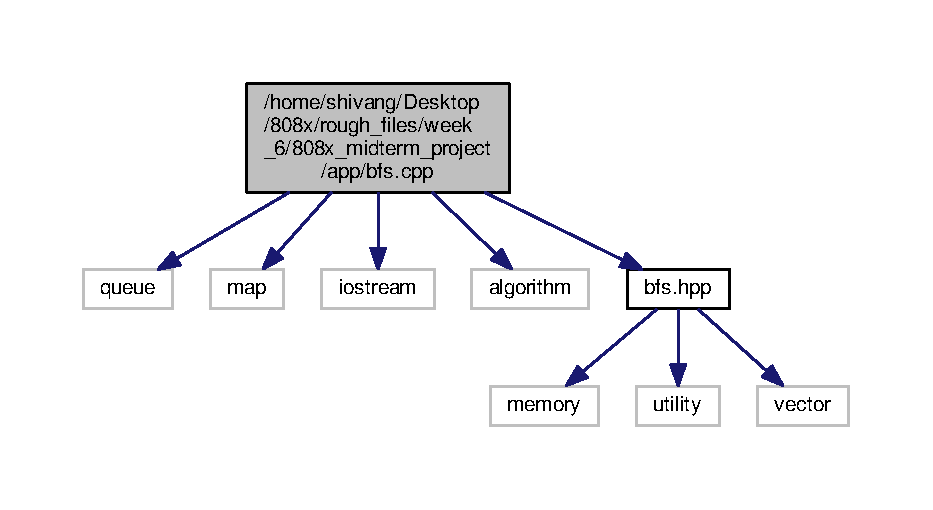
\includegraphics[width=350pt]{bfs_8cpp__incl}
\end{center}
\end{figure}


\subsection{Detailed Description}
D\+E\+S\+C\+R\+I\+P\+T\+I\+ON This file implements \hyperlink{class_bfs}{Bfs} class. 

\begin{DoxyAuthor}{Author}
Shivang Patel 
\end{DoxyAuthor}
\begin{DoxyCopyright}{Copyright}
M\+IT license 
\end{DoxyCopyright}

\hypertarget{main_8cpp}{}\section{/home/shivang/\+Desktop/808x/rough\+\_\+files/week\+\_\+6/808x\+\_\+midterm\+\_\+project/app/main.cpp File Reference}
\label{main_8cpp}\index{/home/shivang/\+Desktop/808x/rough\+\_\+files/week\+\_\+6/808x\+\_\+midterm\+\_\+project/app/main.\+cpp@{/home/shivang/\+Desktop/808x/rough\+\_\+files/week\+\_\+6/808x\+\_\+midterm\+\_\+project/app/main.\+cpp}}


D\+E\+S\+C\+R\+I\+P\+T\+I\+ON This files is the main file which creates object of \hyperlink{class_obstacle__generator}{Obstacle\+\_\+generator} class.  


{\ttfamily \#include $<$iostream$>$}\\*
{\ttfamily \#include $<$obstacle\+\_\+generator.\+hpp$>$}\\*
Include dependency graph for main.\+cpp\+:\nopagebreak
\begin{figure}[H]
\begin{center}
\leavevmode
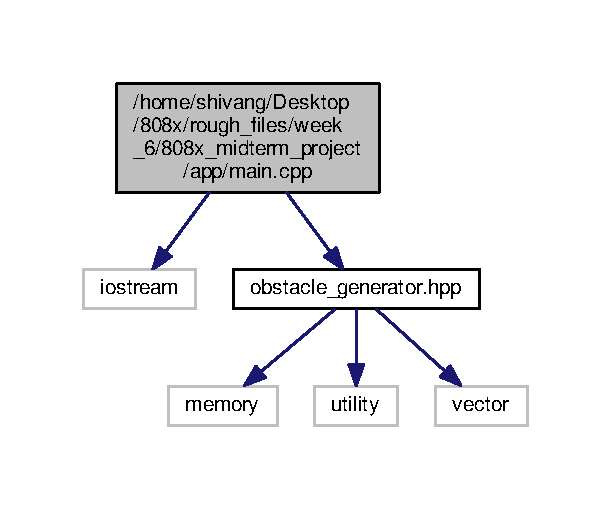
\includegraphics[width=293pt]{main_8cpp__incl}
\end{center}
\end{figure}
\subsection*{Functions}
\begin{DoxyCompactItemize}
\item 
int {\bfseries main} ()\hypertarget{main_8cpp_ae66f6b31b5ad750f1fe042a706a4e3d4}{}\label{main_8cpp_ae66f6b31b5ad750f1fe042a706a4e3d4}

\end{DoxyCompactItemize}


\subsection{Detailed Description}
D\+E\+S\+C\+R\+I\+P\+T\+I\+ON This files is the main file which creates object of \hyperlink{class_obstacle__generator}{Obstacle\+\_\+generator} class. 

\begin{DoxyAuthor}{Author}
Shivang Patel 
\end{DoxyAuthor}
\begin{DoxyCopyright}{Copyright}
M\+IT license 
\end{DoxyCopyright}

\hypertarget{obstacle__generator_8cpp}{}\section{/home/shivang/\+Desktop/808x/rough\+\_\+files/week\+\_\+6/808x\+\_\+midterm\+\_\+project/app/obstacle\+\_\+generator.cpp File Reference}
\label{obstacle__generator_8cpp}\index{/home/shivang/\+Desktop/808x/rough\+\_\+files/week\+\_\+6/808x\+\_\+midterm\+\_\+project/app/obstacle\+\_\+generator.\+cpp@{/home/shivang/\+Desktop/808x/rough\+\_\+files/week\+\_\+6/808x\+\_\+midterm\+\_\+project/app/obstacle\+\_\+generator.\+cpp}}


D\+E\+S\+C\+R\+I\+P\+T\+I\+ON This files implements the class \hyperlink{class_obstacle__generator}{Obstacle\+\_\+generator}.  


{\ttfamily \#include $<$iostream$>$}\\*
{\ttfamily \#include $<$cmath$>$}\\*
{\ttfamily \#include $<$bfs.\+hpp$>$}\\*
{\ttfamily \#include $<$obstacle\+\_\+generator.\+hpp$>$}\\*
{\ttfamily \#include $<$sdl\+\_\+wrapper.\+hpp$>$}\\*
Include dependency graph for obstacle\+\_\+generator.\+cpp\+:\nopagebreak
\begin{figure}[H]
\begin{center}
\leavevmode
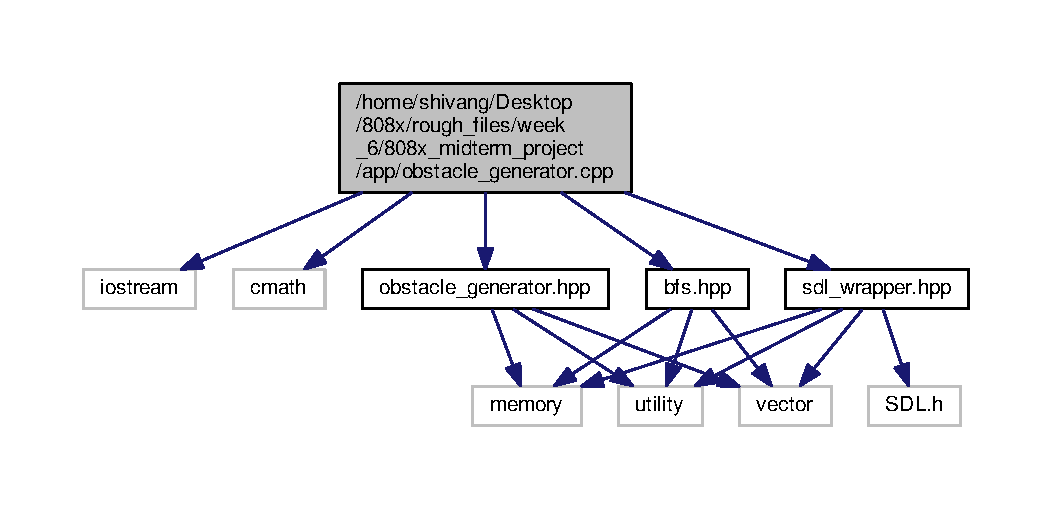
\includegraphics[width=350pt]{obstacle__generator_8cpp__incl}
\end{center}
\end{figure}


\subsection{Detailed Description}
D\+E\+S\+C\+R\+I\+P\+T\+I\+ON This files implements the class \hyperlink{class_obstacle__generator}{Obstacle\+\_\+generator}. 

\begin{DoxyAuthor}{Author}
Shivang Patel 
\end{DoxyAuthor}
\begin{DoxyCopyright}{Copyright}
M\+IT license 
\end{DoxyCopyright}

\hypertarget{sdl__wrapper_8cpp}{}\section{/home/shivang/\+Desktop/808x/rough\+\_\+files/week\+\_\+6/808x\+\_\+midterm\+\_\+project/app/sdl\+\_\+wrapper.cpp File Reference}
\label{sdl__wrapper_8cpp}\index{/home/shivang/\+Desktop/808x/rough\+\_\+files/week\+\_\+6/808x\+\_\+midterm\+\_\+project/app/sdl\+\_\+wrapper.\+cpp@{/home/shivang/\+Desktop/808x/rough\+\_\+files/week\+\_\+6/808x\+\_\+midterm\+\_\+project/app/sdl\+\_\+wrapper.\+cpp}}


D\+E\+S\+C\+R\+I\+P\+T\+I\+ON This files implements the class \hyperlink{class_sdl__wrapper}{Sdl\+\_\+wrapper}.  


{\ttfamily \#include $<$sdl\+\_\+wrapper.\+hpp$>$}\\*
Include dependency graph for sdl\+\_\+wrapper.\+cpp\+:\nopagebreak
\begin{figure}[H]
\begin{center}
\leavevmode
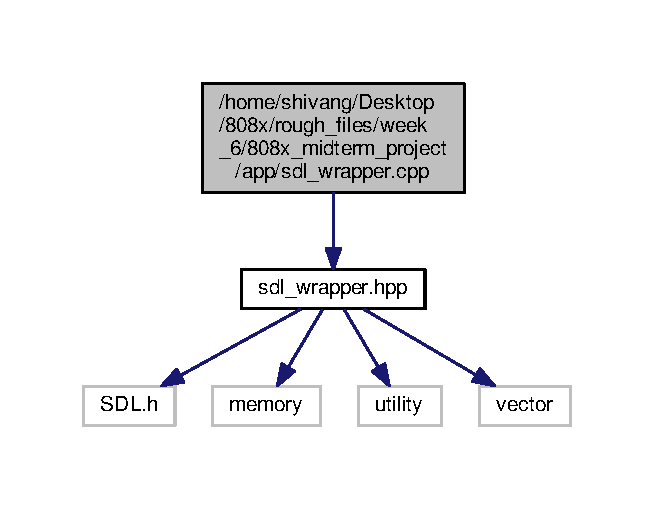
\includegraphics[width=314pt]{sdl__wrapper_8cpp__incl}
\end{center}
\end{figure}


\subsection{Detailed Description}
D\+E\+S\+C\+R\+I\+P\+T\+I\+ON This files implements the class \hyperlink{class_sdl__wrapper}{Sdl\+\_\+wrapper}. 

\begin{DoxyAuthor}{Author}
Shivang Patel 
\end{DoxyAuthor}
\begin{DoxyCopyright}{Copyright}
M\+IT license 
\end{DoxyCopyright}

\hypertarget{bfs_8hpp}{}\section{/home/shivang/\+Desktop/808x/rough\+\_\+files/week\+\_\+6/808x\+\_\+midterm\+\_\+project/include/bfs.hpp File Reference}
\label{bfs_8hpp}\index{/home/shivang/\+Desktop/808x/rough\+\_\+files/week\+\_\+6/808x\+\_\+midterm\+\_\+project/include/bfs.\+hpp@{/home/shivang/\+Desktop/808x/rough\+\_\+files/week\+\_\+6/808x\+\_\+midterm\+\_\+project/include/bfs.\+hpp}}


D\+E\+S\+C\+R\+I\+P\+T\+I\+ON Header file for the class \hyperlink{class_bfs}{Bfs}. \hyperlink{class_bfs}{Bfs} class implements a planning algorithm B\+FS. Breadth First Search algorithm is used for traversing as well as searching. It starts at root and explores all the neighbor nodes at current depth before moving to next depth untill it finds the required thing, or traverse to the goal point respectively.  


{\ttfamily \#include $<$memory$>$}\\*
{\ttfamily \#include $<$utility$>$}\\*
{\ttfamily \#include $<$vector$>$}\\*
Include dependency graph for bfs.\+hpp\+:\nopagebreak
\begin{figure}[H]
\begin{center}
\leavevmode
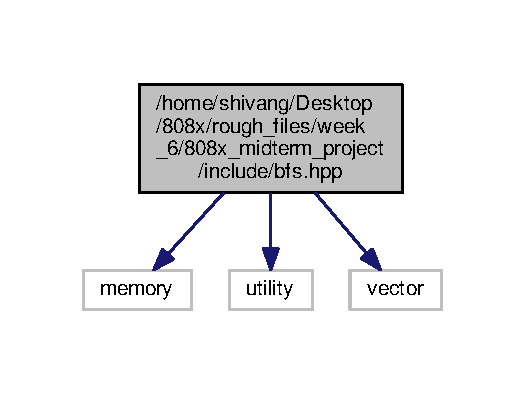
\includegraphics[width=252pt]{bfs_8hpp__incl}
\end{center}
\end{figure}
This graph shows which files directly or indirectly include this file\+:\nopagebreak
\begin{figure}[H]
\begin{center}
\leavevmode
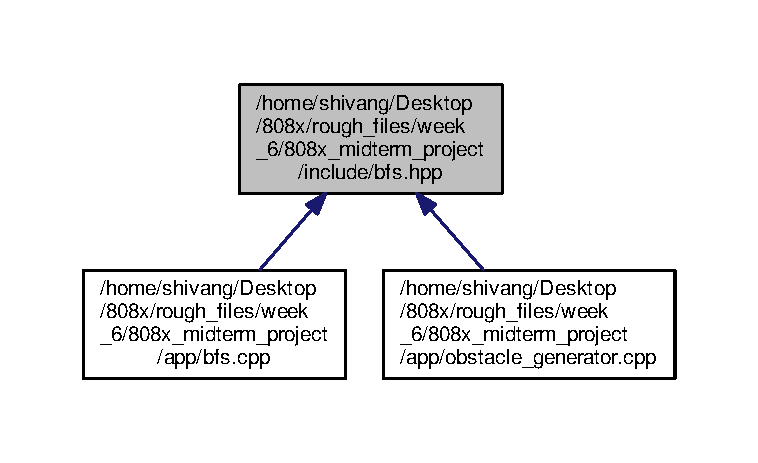
\includegraphics[width=350pt]{bfs_8hpp__dep__incl}
\end{center}
\end{figure}
\subsection*{Classes}
\begin{DoxyCompactItemize}
\item 
class \hyperlink{class_bfs}{Bfs}
\begin{DoxyCompactList}\small\item\em \hyperlink{class_bfs}{Bfs} class which is used to find stortest path possible by using B\+FS algorithm. \end{DoxyCompactList}\end{DoxyCompactItemize}


\subsection{Detailed Description}
D\+E\+S\+C\+R\+I\+P\+T\+I\+ON Header file for the class \hyperlink{class_bfs}{Bfs}. \hyperlink{class_bfs}{Bfs} class implements a planning algorithm B\+FS. Breadth First Search algorithm is used for traversing as well as searching. It starts at root and explores all the neighbor nodes at current depth before moving to next depth untill it finds the required thing, or traverse to the goal point respectively. 

\begin{DoxyAuthor}{Author}
Shivang Patel 
\end{DoxyAuthor}
\begin{DoxyCopyright}{Copyright}
M\+IT license 
\end{DoxyCopyright}

\hypertarget{obstacle__generator_8hpp}{}\section{/home/shivang/\+Desktop/808x/rough\+\_\+files/week\+\_\+6/808x\+\_\+midterm\+\_\+project/include/obstacle\+\_\+generator.hpp File Reference}
\label{obstacle__generator_8hpp}\index{/home/shivang/\+Desktop/808x/rough\+\_\+files/week\+\_\+6/808x\+\_\+midterm\+\_\+project/include/obstacle\+\_\+generator.\+hpp@{/home/shivang/\+Desktop/808x/rough\+\_\+files/week\+\_\+6/808x\+\_\+midterm\+\_\+project/include/obstacle\+\_\+generator.\+hpp}}


D\+E\+S\+C\+R\+I\+P\+T\+I\+ON This class will artificially generate obstacle, throught methods, for B\+FS algorithm. This class will act as Acme\textquotesingle{}s high level planner\textquotesingle{}s input to \hyperlink{class_bfs}{Bfs} module.  


{\ttfamily \#include $<$memory$>$}\\*
{\ttfamily \#include $<$utility$>$}\\*
{\ttfamily \#include $<$vector$>$}\\*
Include dependency graph for obstacle\+\_\+generator.\+hpp\+:\nopagebreak
\begin{figure}[H]
\begin{center}
\leavevmode
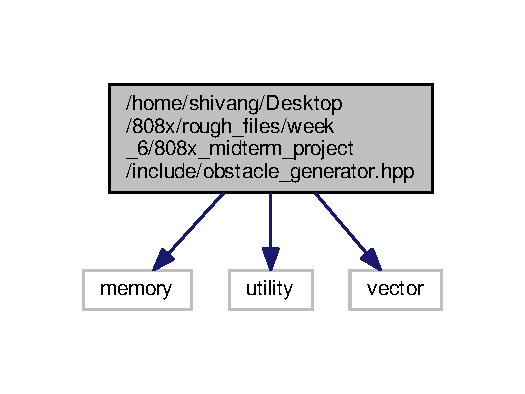
\includegraphics[width=252pt]{obstacle__generator_8hpp__incl}
\end{center}
\end{figure}
This graph shows which files directly or indirectly include this file\+:\nopagebreak
\begin{figure}[H]
\begin{center}
\leavevmode
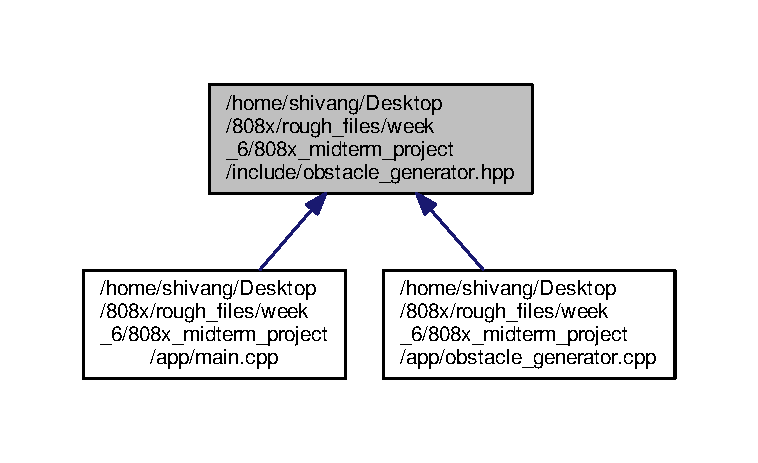
\includegraphics[width=350pt]{obstacle__generator_8hpp__dep__incl}
\end{center}
\end{figure}
\subsection*{Classes}
\begin{DoxyCompactItemize}
\item 
class \hyperlink{class_obstacle__generator}{Obstacle\+\_\+generator}
\begin{DoxyCompactList}\small\item\em This class will mimic the Acme\textquotesingle{}s high level planner\textquotesingle{}s . This class will provide the hight and width of the area, obstacle space and start -\/ goal points. And evoke the planner. \end{DoxyCompactList}\end{DoxyCompactItemize}


\subsection{Detailed Description}
D\+E\+S\+C\+R\+I\+P\+T\+I\+ON This class will artificially generate obstacle, throught methods, for B\+FS algorithm. This class will act as Acme\textquotesingle{}s high level planner\textquotesingle{}s input to \hyperlink{class_bfs}{Bfs} module. 

\begin{DoxyAuthor}{Author}
Shivang Patel 
\end{DoxyAuthor}
\begin{DoxyCopyright}{Copyright}
M\+IT license 
\end{DoxyCopyright}

\hypertarget{sdl__wrapper_8hpp}{}\section{/home/shivang/\+Desktop/808x/rough\+\_\+files/week\+\_\+6/808x\+\_\+midterm\+\_\+project/include/sdl\+\_\+wrapper.hpp File Reference}
\label{sdl__wrapper_8hpp}\index{/home/shivang/\+Desktop/808x/rough\+\_\+files/week\+\_\+6/808x\+\_\+midterm\+\_\+project/include/sdl\+\_\+wrapper.\+hpp@{/home/shivang/\+Desktop/808x/rough\+\_\+files/week\+\_\+6/808x\+\_\+midterm\+\_\+project/include/sdl\+\_\+wrapper.\+hpp}}


D\+E\+S\+C\+R\+I\+P\+T\+I\+ON Header file for the class \char`\"{}\+Sdl\+\_\+wrapper\char`\"{}. This class act as wrapper of original S\+DL library for C++. It encaptulates enough functionality from the library for visual of environment, on which B\+FS has been used, and path it has generated. Information about path and environment, obstacles and space size, will be recieved externally from \hyperlink{class_obstacle__generator}{Obstacle\+\_\+generator} class and this will generate visuals accordingly.  


{\ttfamily \#include \char`\"{}S\+D\+L.\+h\char`\"{}}\\*
{\ttfamily \#include $<$memory$>$}\\*
{\ttfamily \#include $<$utility$>$}\\*
{\ttfamily \#include $<$vector$>$}\\*
Include dependency graph for sdl\+\_\+wrapper.\+hpp\+:\nopagebreak
\begin{figure}[H]
\begin{center}
\leavevmode
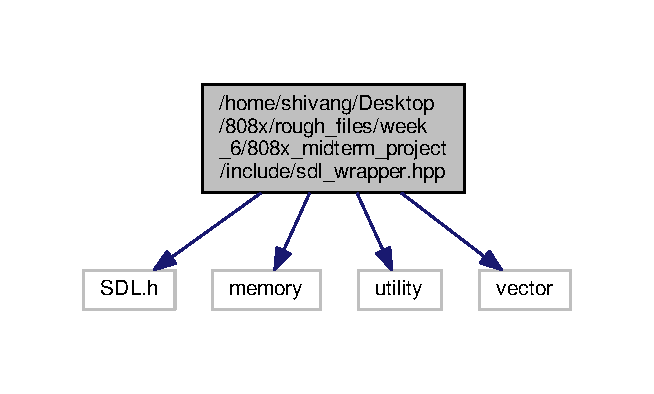
\includegraphics[width=314pt]{sdl__wrapper_8hpp__incl}
\end{center}
\end{figure}
This graph shows which files directly or indirectly include this file\+:
\nopagebreak
\begin{figure}[H]
\begin{center}
\leavevmode
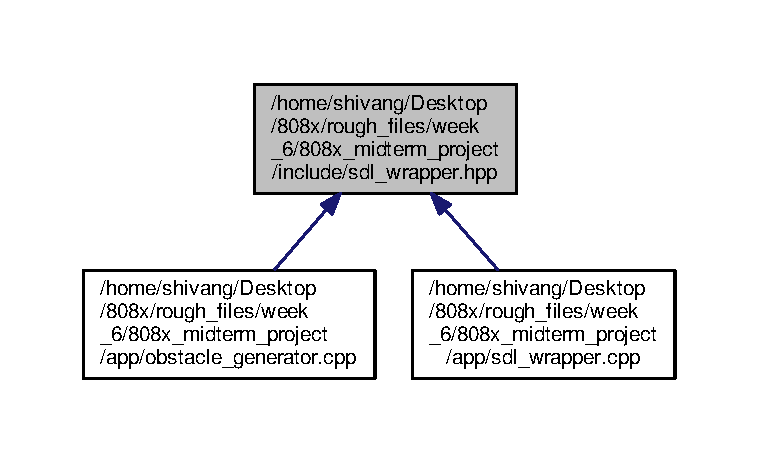
\includegraphics[width=350pt]{sdl__wrapper_8hpp__dep__incl}
\end{center}
\end{figure}
\subsection*{Classes}
\begin{DoxyCompactItemize}
\item 
class \hyperlink{class_sdl__wrapper}{Sdl\+\_\+wrapper}
\begin{DoxyCompactList}\small\item\em S\+DL library wrapper class for visulization of the B\+FS algorithm through the \hyperlink{class_bfs}{Bfs} class. This class will accept all the information regarding the environment and path for plotting them in nice visuals. \end{DoxyCompactList}\end{DoxyCompactItemize}


\subsection{Detailed Description}
D\+E\+S\+C\+R\+I\+P\+T\+I\+ON Header file for the class \char`\"{}\+Sdl\+\_\+wrapper\char`\"{}. This class act as wrapper of original S\+DL library for C++. It encaptulates enough functionality from the library for visual of environment, on which B\+FS has been used, and path it has generated. Information about path and environment, obstacles and space size, will be recieved externally from \hyperlink{class_obstacle__generator}{Obstacle\+\_\+generator} class and this will generate visuals accordingly. 

\begin{DoxyAuthor}{Author}
Shivang Patel 
\end{DoxyAuthor}
\begin{DoxyCopyright}{Copyright}
M\+IT license 
\end{DoxyCopyright}

%--- End generated contents ---

% Index
\backmatter
\newpage
\phantomsection
\clearemptydoublepage
\addcontentsline{toc}{chapter}{Index}
\printindex

\end{document}
